\documentclass[a4paper]{article}
\usepackage[a4paper, total={6.5in, 10in}]{geometry}
\usepackage[english]{babel}
\usepackage[utf8]{inputenc}
\usepackage{amsmath}
\usepackage{graphicx}
\usepackage{multirow}
\usepackage{graphicx}
\usepackage{caption}
\usepackage{subcaption}
\usepackage{floatrow}
\restylefloat{table}
\usepackage[colorinlistoftodos]{todonotes}
\usepackage{float}
\title{Vector-Valued Image Regularization with PDEs}

\author{Meet Kathiriya, Shreyas Pimpalgaonkar, Saiteja Talluri \\ 160050001,160050024,160050098}

\date{\today}

\begin{document}
\maketitle

\begin{abstract}

We focussed on techiniques for vector-valued image regularization, based on variational methods and PDEs. We performed denoising, image reconstruction, inpainting, magnification and flow visualization on color images using these techinques and presented our results and conclusions.
\end{abstract}

\section{Theory}
\label{sec:theory}
\hspace{5mm}The problem of image regularisation can be solved by three interconnected models of functional \\ minimisation, divergence expressions and oriented laplacians. 

The structure tensor is used here, and it's eigen vectors represent directions of maximum variation. Therefore, the problem can be formulated as minimising the generalised functional representing the variation in the image using the eigen vectors as follows
$$\min_{I:\Omega\to\mathcal{R}^{n}} E(I) = \int_{\Omega} \psi(\lambda_{+},\lambda_{-})\,d\Omega$$

 The above equation can be converted to the divergence of a diffusion matrix with gradient of the Image channel by using Euler-Lagrange theorem, heat equations, orthogonality of eigen vectors and simple partial differential equation chain rules as done in the appendix 1 of the original paper. 
        $$\frac{\partial I_i}{\partial t} = div ( D \nabla I )          \qquad  (i = 1..n) $$ 
        $$ \textbf{D} = \frac{\partial \psi}{\partial \lambda_+} \theta_+ \theta_+^T  +  \frac{\partial \psi}{\partial \lambda_-} \theta_- \theta_-^T$$
    where $n$ is the number of channels and $\theta_+,\theta_-$ are the eigen vectors of the structure tensor. If a $\psi$ exists, eigenvalues of the divergence tensor D can be seen it's gradient and obtaining $I_i$ is easy for every channel.
    
The oriented laplacian equation can be written as the following PDE
$$\frac { \partial I _ { i } } { \partial t } = c _ { 1 } I _ { i \epsilon \varepsilon } + c _ { 2 } I _ { i m } = \operatorname { trace } \left( \mathbf { T } H _ { i } \right)$$
 $$ I _ { i ( t ) } = I _ { i _ { ( t = 0 ) } } * G ^ { ( \mathbf { T } , t ) }$$ 
where $*$ stands for the convolution with the oriented Gaussian kernel 
$$G ^ { ( \mathbf { T } , t ) } ( \mathbf { x } ) = \frac { 1 } { 4 \pi t } \exp \left( - \frac { \mathbf { x } ^ { T } \mathbf { T } ^ { - 1 } \mathbf { x } } { 4 t } \right) \quad \text { with } \quad \mathbf { x } = ( x \quad y ) ^ { T }$$

$$\frac { \partial I _ { i } } { \partial t } = \operatorname { trace } \left( \mathbf { T } \mathbf { H } _ { i } \right) \quad ( i = 1 . . n )$$

where $\textbf{T}$ is the tensor field defined pointwise as 
    
$$\mathbf { T } = f _ { - } \left( \sqrt { \lambda _ { + } ^ { * } + \lambda _ { - } ^ { * } } \right) \theta _ { - } ^ { * } \theta _ { - } ^ { * T } + f _ { + } \left( \sqrt { \lambda _ { + } ^ { * } + \lambda _ { - } ^ { * } } \right) \theta _ { + } ^ { * } \theta _ { + } ^ { * } T$$

where $\lambda_{\pm}^*$ and $\theta_{\pm}^*$ are defined to be the spectral elements of $G_\sigma = G * G_{\sigma'}$ , a Gaussian smoothed version of the structure tensor G, allowing us to retrieve a more coherent vector geometry giving a better approximation of the vector discontinuity directions.  

For our experiments we choose, $f _ { + } ( s ) = \frac { 1 } { 1 + s ^ { 2 } } .\text { and } f _ { - } ( s ) = \frac { 1 } { \sqrt { 1 + s ^ { 2 } } }$ \newline

Finally, a high level overview of the algorithm is to convolve the image with a gaussian that solves the PDE of Oriented Laplacians with $\textbf{T}$ and $f$ as in the above section. This is equivalent to using the trace formula in section 2.3 and also is proved in the original paper.
    
\pagebreak
\section{Results and Inferences}

\subsection{Image Inpainting}

\begin{figure}[h]
\centering
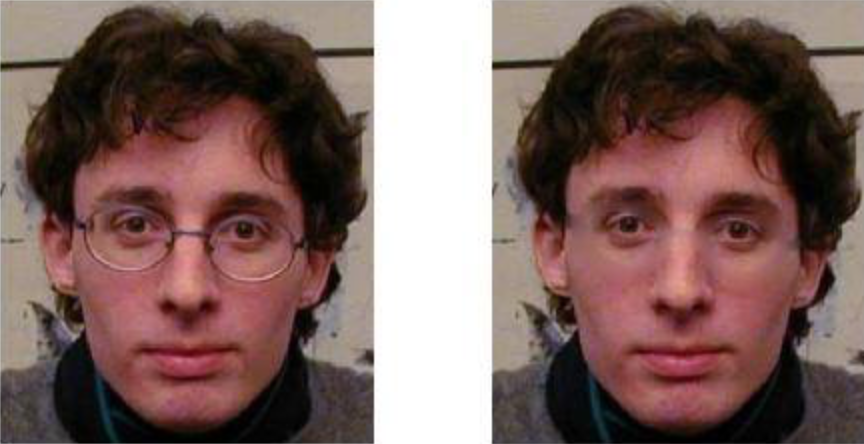
\includegraphics[width=1\textwidth]{glasses.png}
\caption{\label{fig:data} Inpainting with 21x21 neighbourhood, t=5 and 10 iterations}
\end{figure}

\begin{figure}[h]
\centering
\includegraphics[width=1\textwidth]{parrot1.png}
\caption{\label{fig:data} Inpainting with 10x10 neighbourhood, t=2 and 20 iterations}
\end{figure}


\begin{figure}[H]
\centering
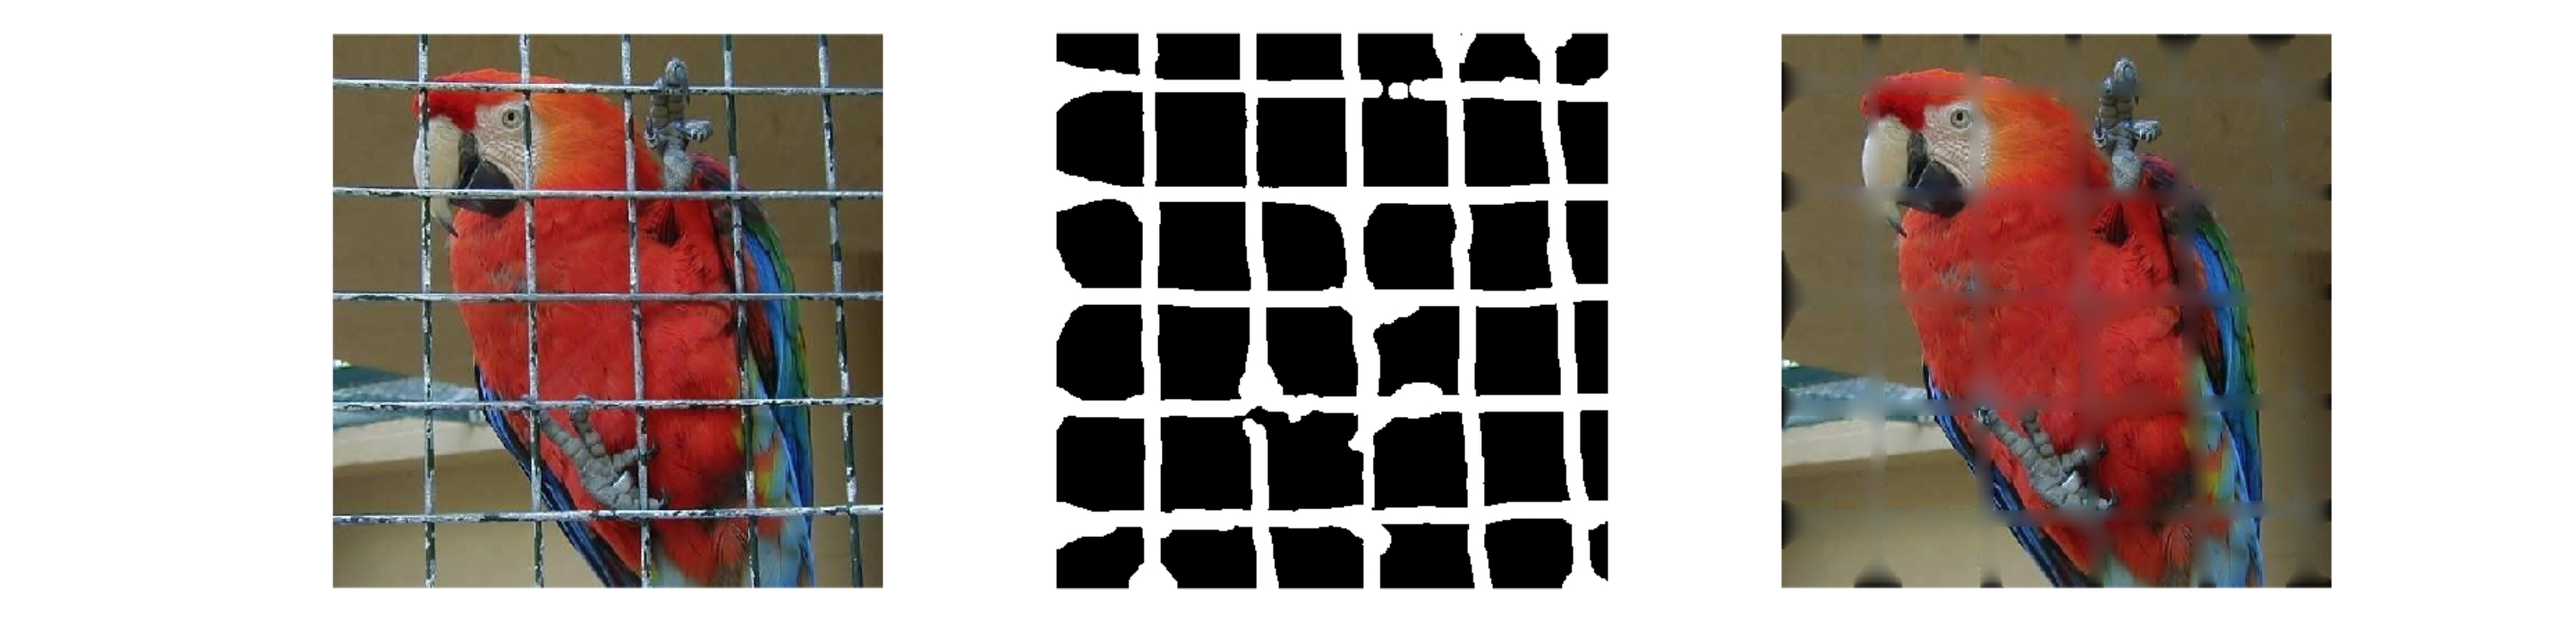
\includegraphics[width=1\textwidth]{redparrot.png}
\caption{\label{fig:data} Inpainting with 20x20 neighbourhood, t=3 and 20 iterations Also the black prints at boundaries and some darker regions in image is due to the fact that the mask we are using is imperfect as it contains more white region at some locations than the cage obstacle in real image.}
\end{figure}

\pagebreak
\subsection{Image Denoising}


\begin{figure}[h]
\centering
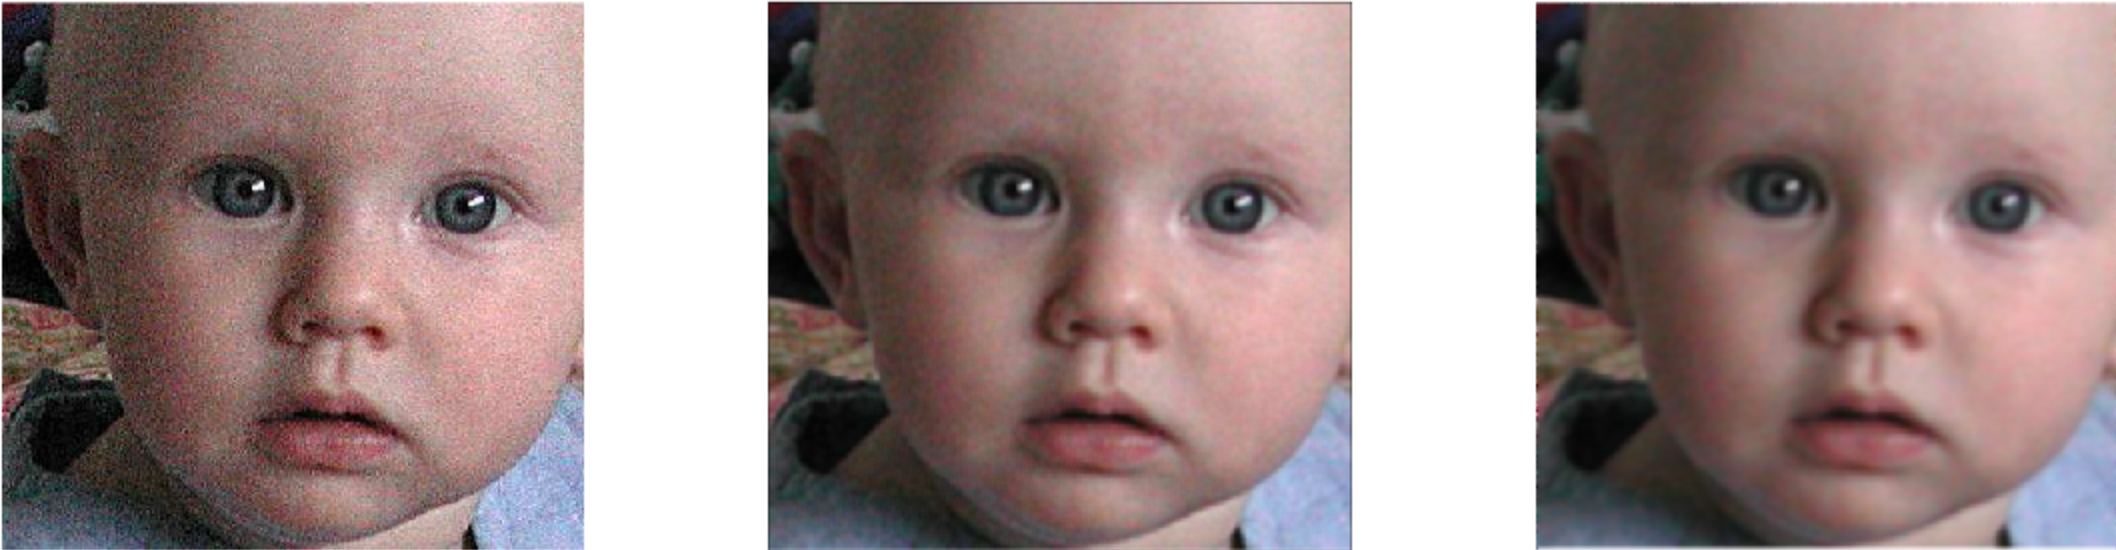
\includegraphics[width=1\textwidth]{baby.png}
\caption{\label{fig:data} From L to R : Noisy image, image filtered with gaussian smoothing with 5x5 kernel, image filtered with PDE regularisation with t=3, 3x3 neighbourhood and 5 iterations - better performance and lower noise especially on left and top parts of the image }
\end{figure}

\begin{figure}[h]
\centering
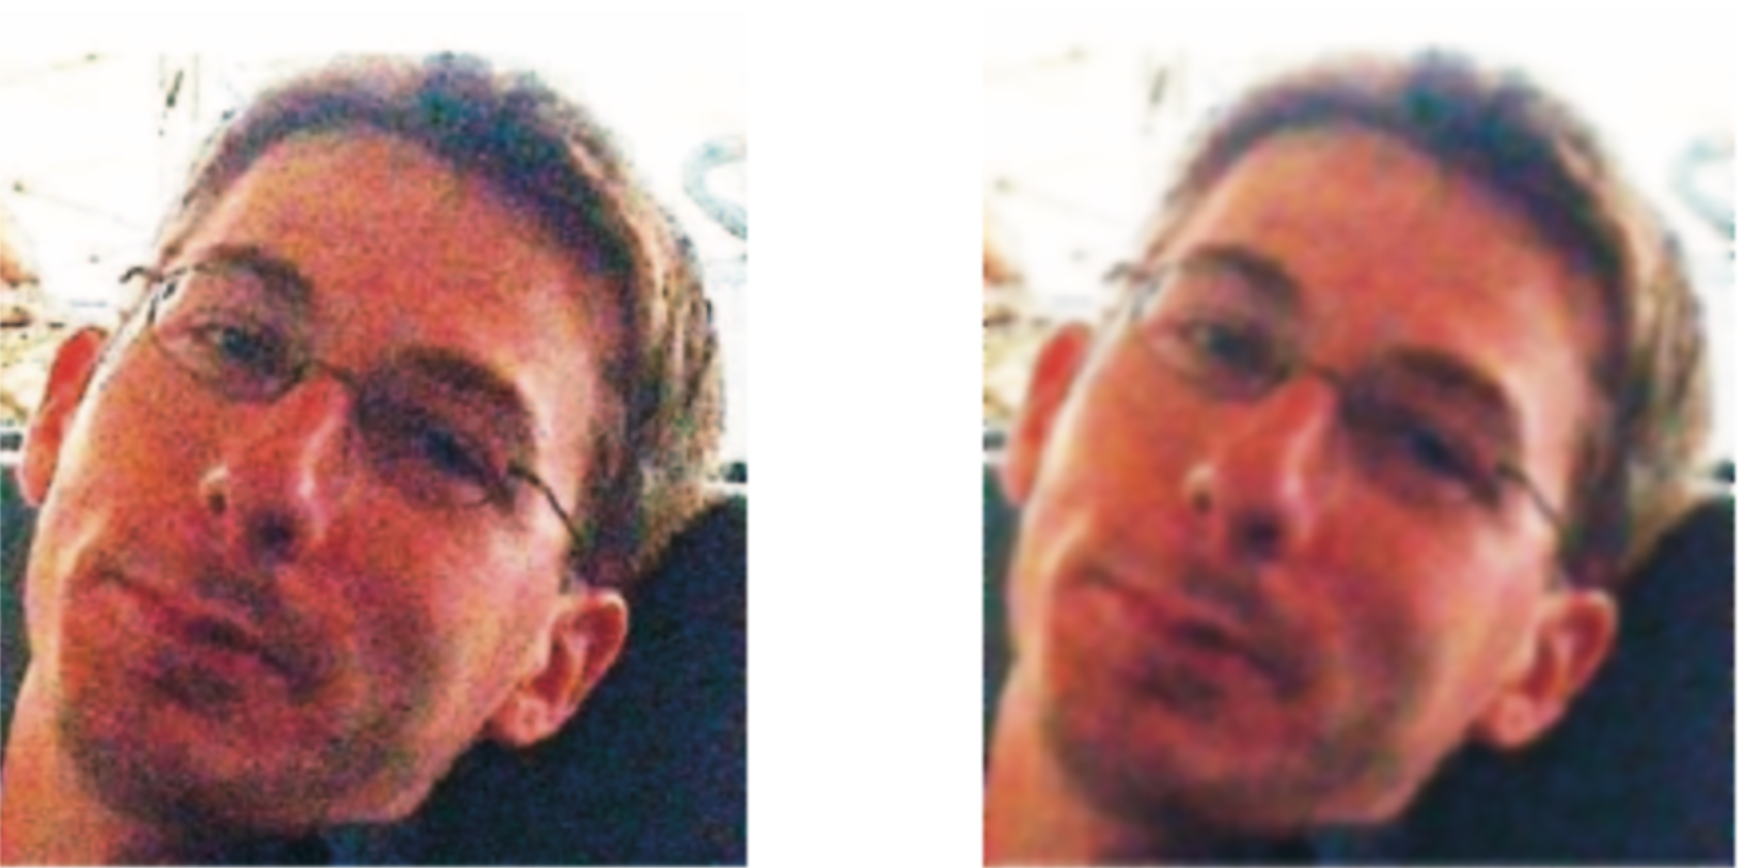
\includegraphics[width=0.8\textwidth,height=0.4\textwidth]{face.png}
\caption{\label{fig:data} From L to R : Noisy image, image filtered with PDE with t=3, 3x3 neighbourhood and 5 iterations }
\end{figure}

\subsection{Image Magnification}

\begin{figure}[H]
\centering
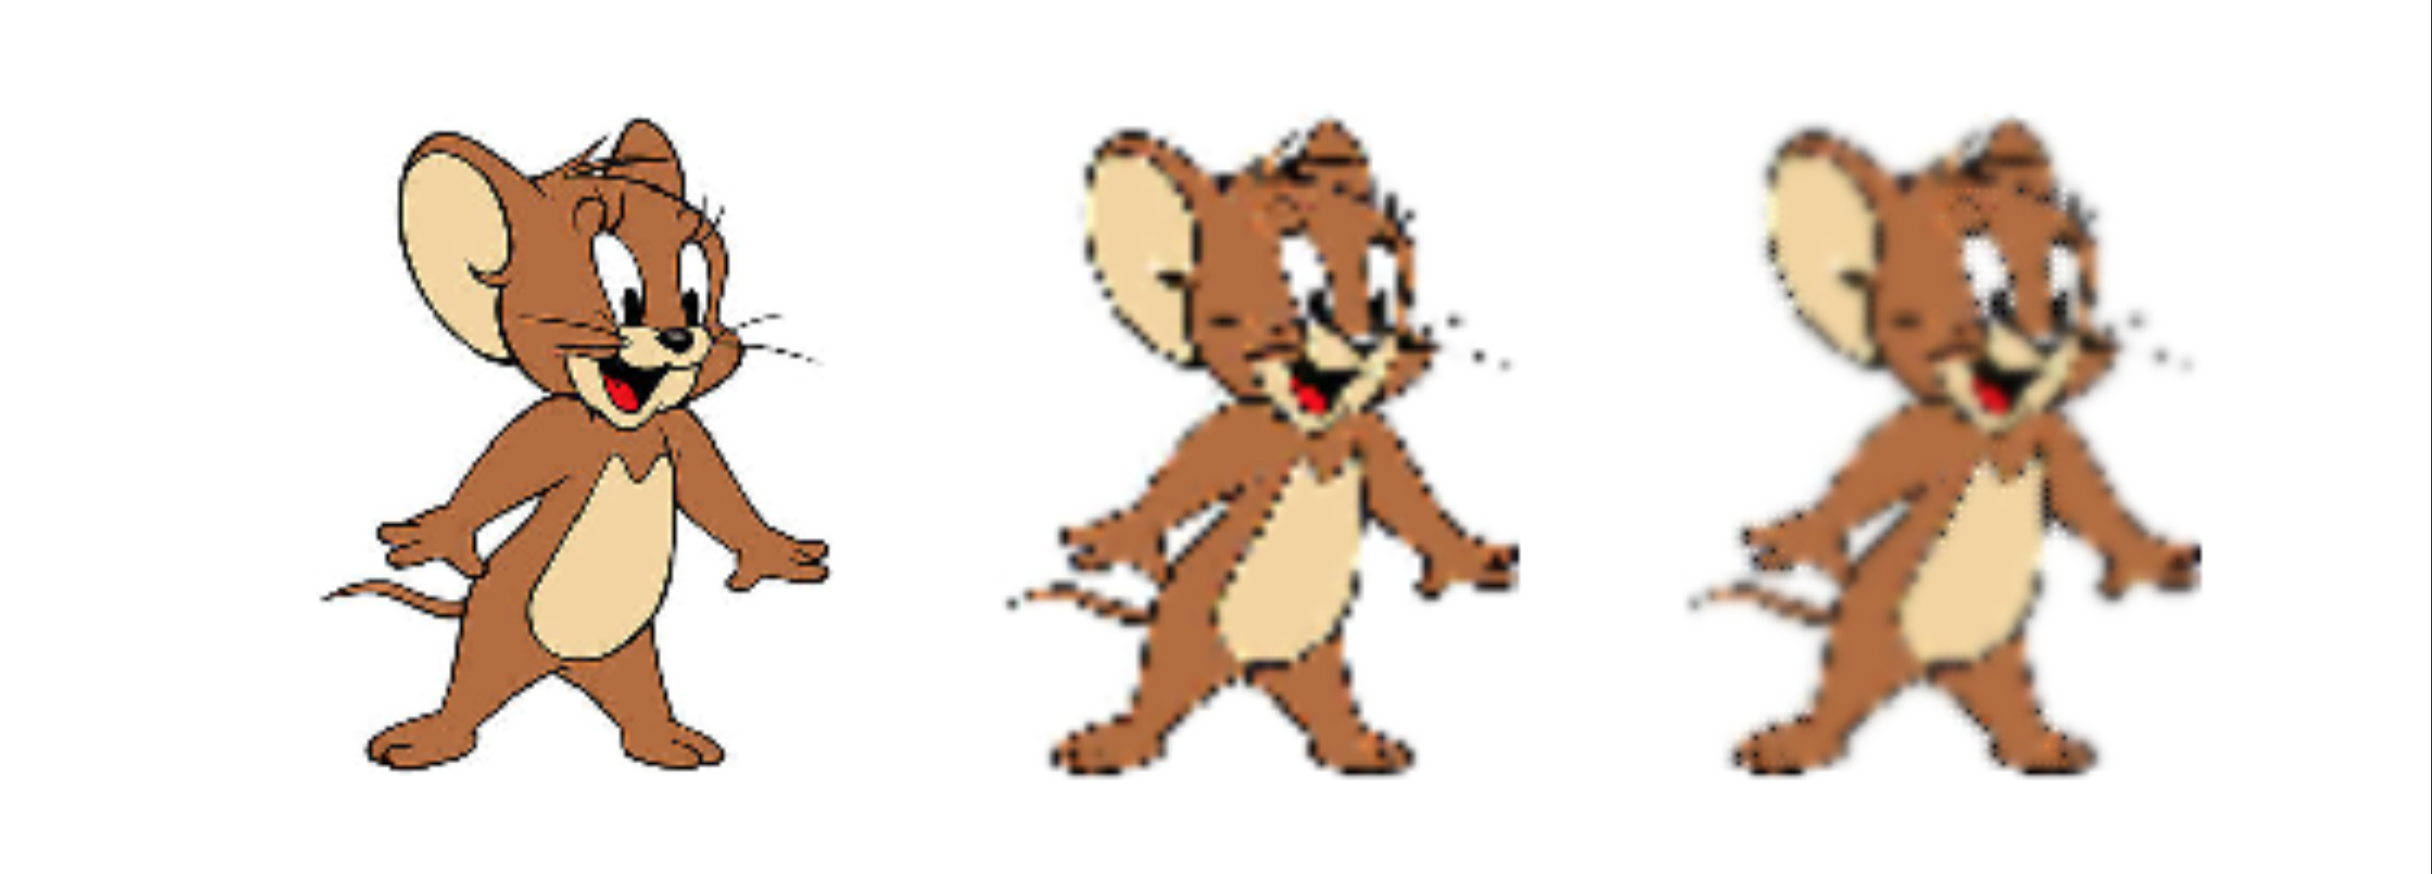
\includegraphics[width=0.8\textwidth]{jerry.png}
\caption{\label{fig:data}
    From L to R : Original Image. This image was downsampled by 4 to serve as input for the two algorithms. Magnified image using bi-linear interpolation, magnified image using PDE regularisation with t=3, 3x3 neighbourhood and 10 iterations. 
}

\end{figure}

\pagebreak

\subsection{Flow Visualisation}

\begin{table}[H]
\caption{Input images, flow vectors and output images, with dt = 0.01, 100 iterations and sobel gradient vectors for Hessian Matrix. Paralallised code, runs much faster compared to others}
\begin{tabular}{c c c}
\includegraphics[width=0.33\textwidth,height=0.4\textwidth]{1} & \includegraphics[width=0.33\textwidth,height=0.4\textwidth]{5} & 
\includegraphics[width=0.33\textwidth,height=0.4\textwidth]{2}\\
\includegraphics[width=0.33\textwidth,height=0.4\textwidth]{4} & \includegraphics[width=0.33\textwidth,height=0.4\textwidth]{6} &
\includegraphics[width=0.33\textwidth,height=0.4\textwidth]{3}
\end{tabular}
\end{table}

\subsection{Image Restoration}


\begin{figure}[H]
\centering
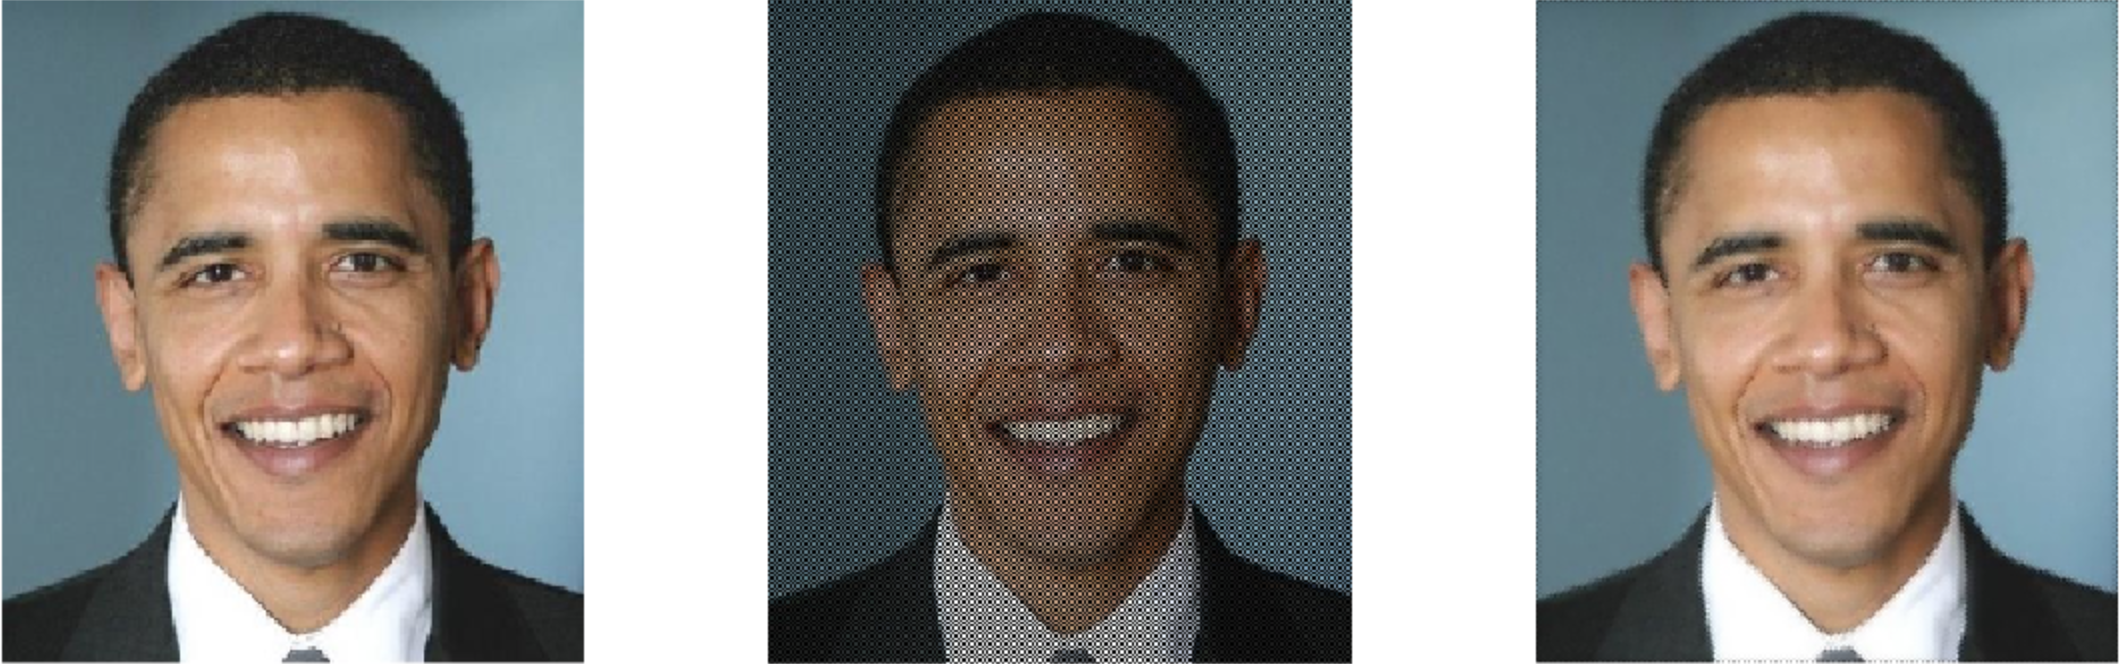
\includegraphics[width=1\textwidth]{obama.png}
\caption{\label{fig:data}
    From L to R : Input Image, image with 50 \% pixels removed in 2x2 granularity, output image with SSIM of 0.995, better than results with median filter. Also, median filter will become less accurate on increasing the box sizes. }

\end{figure}

\begin{figure}[H] \label{frow}
 \begin{floatrow} 
 {\includegraphics[width=0.5\textwidth]{l1}}
 {\includegraphics[width=0.5\textwidth]{l2}}
 \end{floatrow}
 \caption{\label{fig:data} from L to R : image with 50 \% pixels removed and SSIM = 0.23, restored image with t=4, 10 iterations with 3x3 neighbourhood, SSIM = 0.966 with original image}
\end{figure}




\section{Experimental Observations and Conclusions}

\begin{enumerate}
    \item This technique is hard to parallelise in MATLAB as we have to calculate the eigen vectors and eigen values of the  structure tensor at each pixel (The matrix $\textbf{T}$). The MATLAB eig function doesn't provide this functionality. We tried to do this using parfor but it takes too much time to setup the threads and ultimately is slower.
    
    \item Image Inpainting fails drastically as the size of the width of continuous portion of mask increases. Inpainting by this framework is only suitable for removing shapes like cylinders/spheres with small radii. On increasing the width, the lost information is harder to recover due to the high variability in diffusion. Some techniques that specialise in hole filling on the basis of similar patterns like used in Mean Shift Segmentation can be used to give better results. Also, machine learning models can be trained to predict the missing parts, rather than regularisation.
    
    \item This technique performs almost similar to bilateral filtering in denoising images, with a lot more computation overhead.
    
    \item Algorithm follows three main parameters neighbourhood,number of iterations and time. From our experimentation we observed that neighbourhood size highly affects the regularization and it determines amount of smoothing (directly proportional) and edge preservation (indirectly proportional), number of iteration also determines above mentioned image characteristics but they characteristic change start to converge as the number of iteration increases. the time parameter we observed to be least affecting on result as in a very large t worked as a mean filter and very small t there was no significant regularization on image. 
    
    \item While using PDE for image magnification we didn't obtain desired results when the down sampling ratio is high. The possible reason for this could be that we are applying PDE on image magnified with bi-linear interpolation which doesn't retain global features like edges for high down sampling ratios.
    
    \item Flow visualization with PDEs doesn't require calculation of Tensor field at each point unlike denoising and inpainting so with vector manipulations in MATLAB we could very efficiently compute it if the Field vector is not dependent on local variations at each pixel. 
    
\end{enumerate}

\begin{thebibliography}{9}
D. Tschumperle ́ and R. Deriche, “Vector-valued image regularization with PDE’s: A common framework for different applications,” IEEE Trans. PAMI, vol. 27, no. 4, pp. 506–517, 2005. 
\end{thebibliography}
\end{document}